\section{Registration}

{
\setbeamertemplate{background}{}
\setbeamertemplate{navigation symbols}{}
\setbeamercolor{background canvas}{bg={black}}
\color{white}
\begin{frame}[plain]
\fontsize{36pt}{36pt}\selectfont
\center
\begin{center}
Refactored Registration Framework
\end{center}

\fontsize{12pt}{12pt}\selectfont
\begin{center}
Insight Software Consortium
\end{center}
\vskip12pt
\begin{center}
 PICSL @ University of Pennsylvania 
\end{center}
\vskip12pt
\begin{center}
 Brian Avants, Nicholas Tustison, Gang Song, \\ 
Baohua Wu, Michael Stauffer, James C. Gee
\end{center}
\end{frame}
}

\subsection{Refactoring overview}

 \centeredlargetext{white}{black}{
\centering Unified multi-core framework + parameter-estimation
% 
\includegraphics[height=1.8in]{../Art/ITKv4}
 }


\begin{comment}
{

\begin{frame}
\frametitle{Image Registration Refactoring}
\Large
\begin{itemize}
\item Unify frameworks: local \& global 
\pause
\item New metrics and transform operations for vectors \&  tensors
\pause 
\item Composite Transform
\pause
\item Unbiased registration
\pause
\item Multi-threading 
\pause 
\item Automated parameter scaling
\end{itemize}
\end{frame}

\begin{frame}
\frametitle{Unified framework}
\Large
\begin{itemize}
\item Local \& global transforms treated the same in resampler
\item Both types available to (revised) optimizers
\item Revised metrics optimized for these operations
\item Tensors, vector, scalars treated transparently
\end{itemize}
\end{frame}
}
\end{comment}

 \centeredlargetext{white}{black}{
ITK v3 framework
\vskip20pt
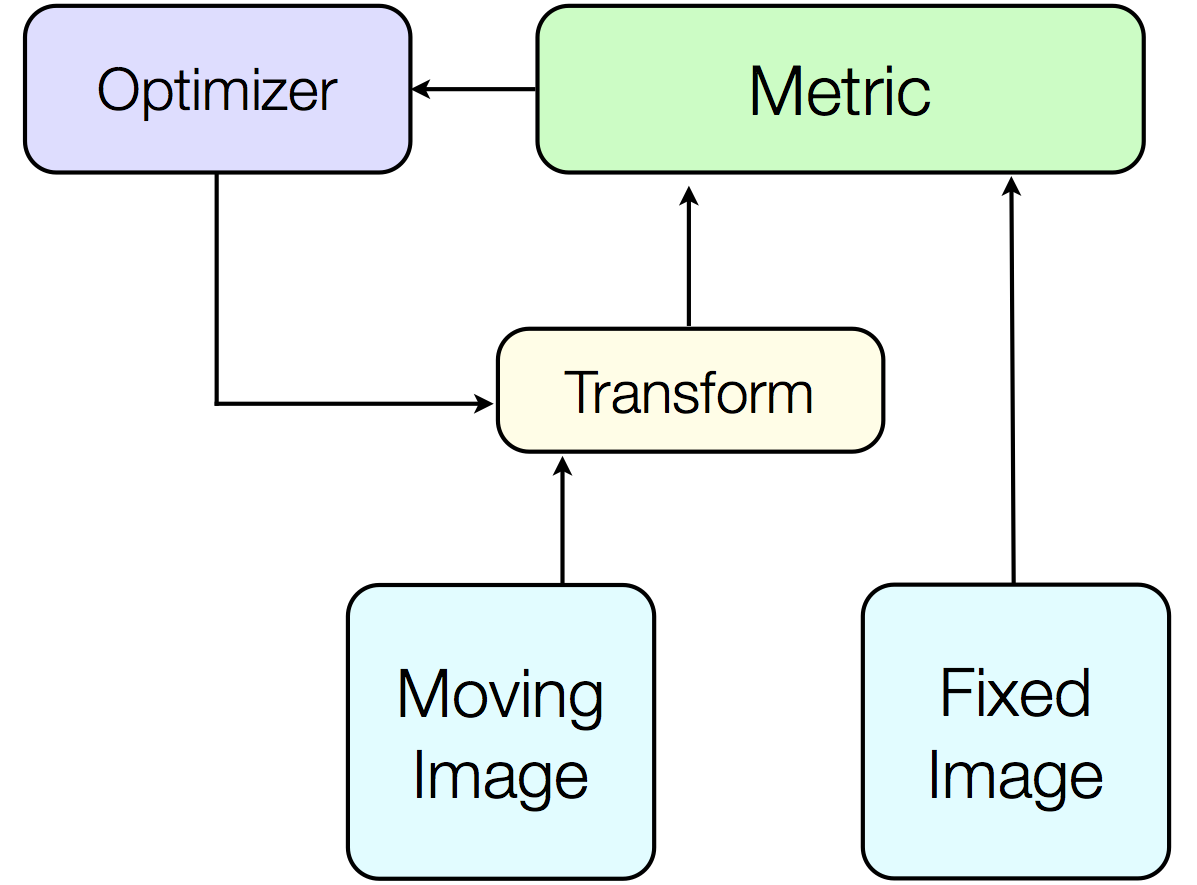
\includegraphics[height=2.2in]{../Art/itkv3reg}
 }

 \centeredlargetext{white}{black}{
ITK v4 framework
\vskip20pt
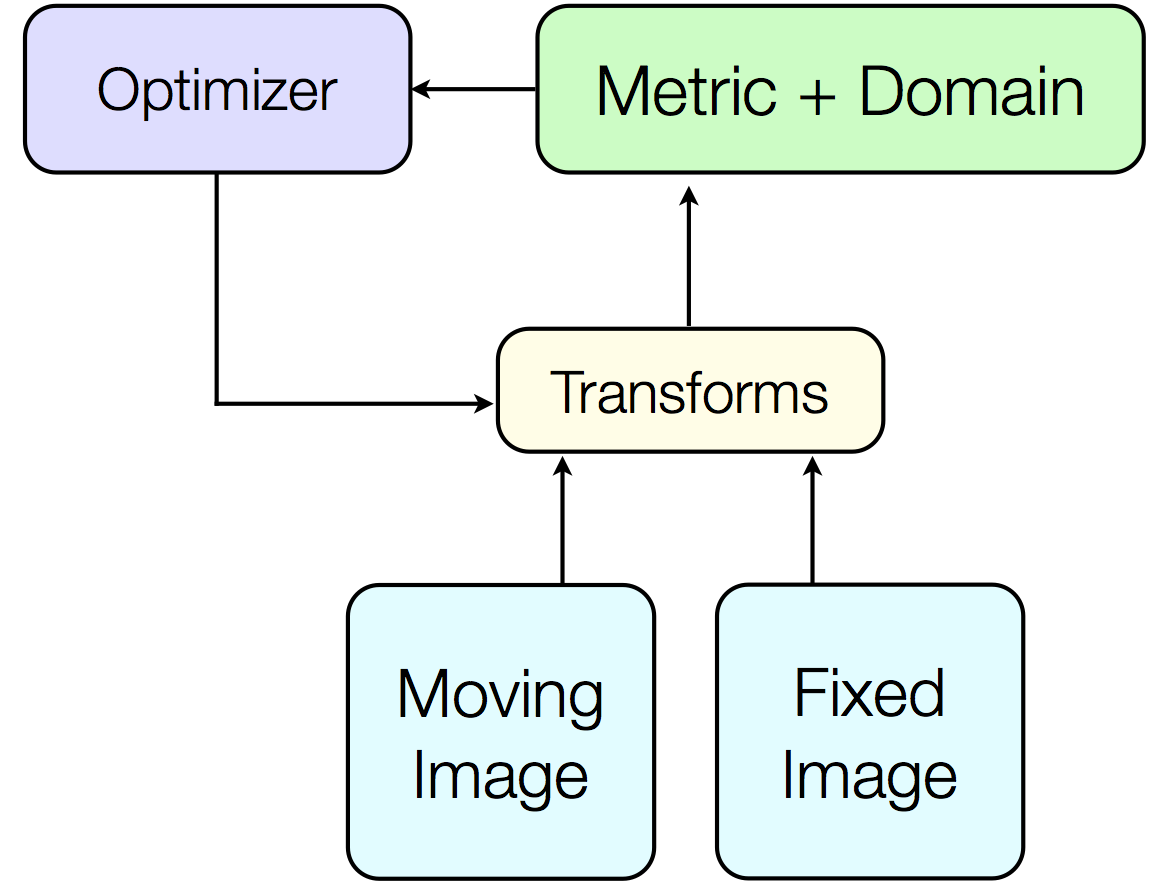
\includegraphics[height=2.2in]{../Art/itkv4reg}
 }

\begin{frame}
\frametitle{Composite transformations}
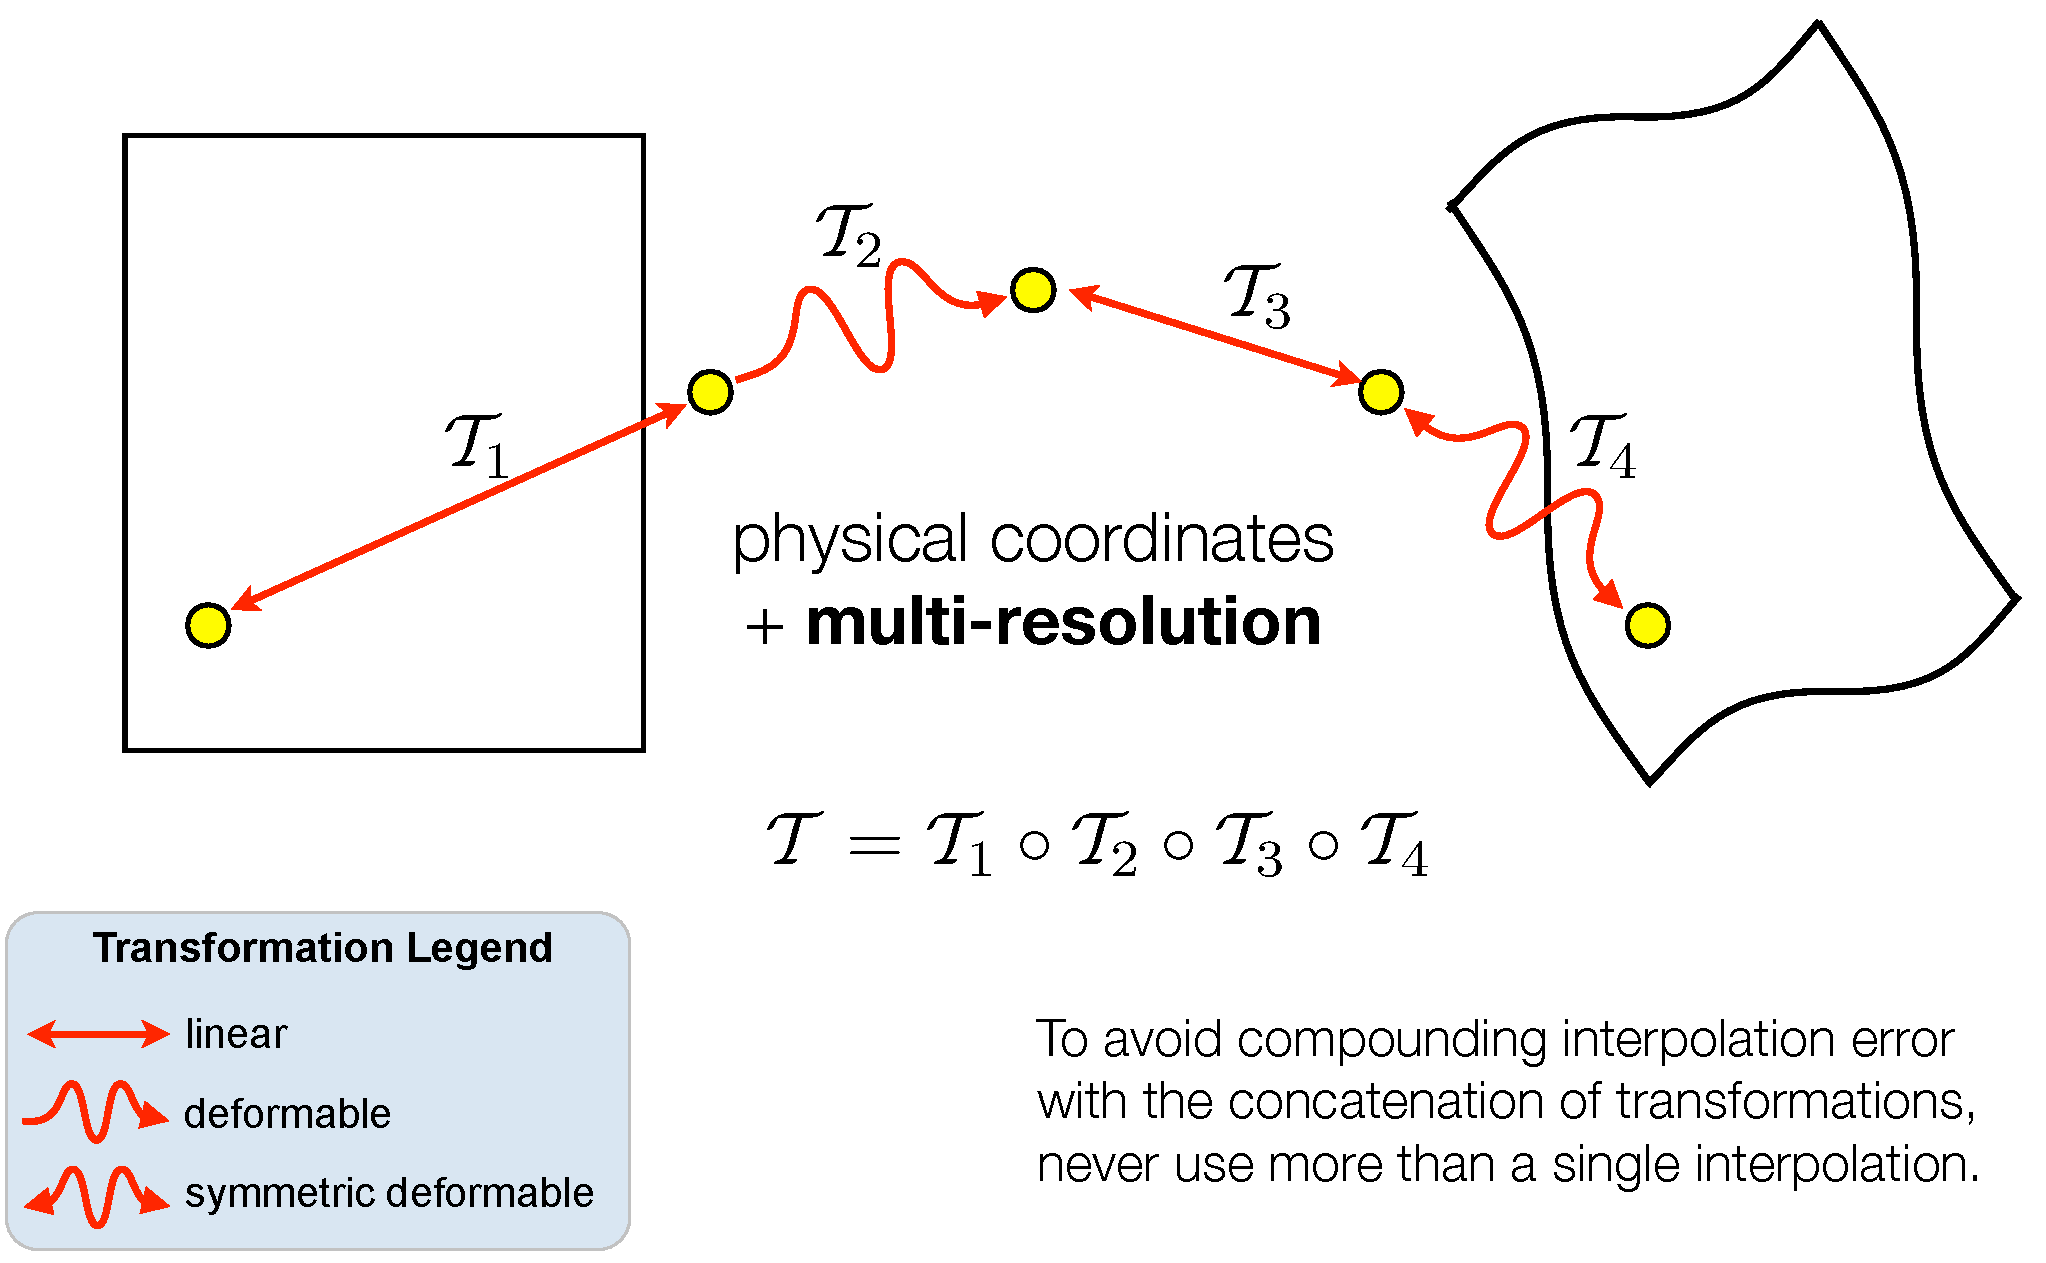
\includegraphics[height=2.5in]{../Art/composite}
\end{frame}

